\label{sec:ecology}

\subsection{Назначение двигателя}
\label{sub:ecology_engine_purpose}

Двигатель предназначен для использования в качестве привода нагнетателя на линейных компрессорных станциях природного газа.

Двигатель выполнен трехвальным со свободной турбиной.

Мощность – 16 МВт.

Основные части: компрессор низкого давления (КНД), компрессор высокого давления (КВД), камера сгорания (КС), турбина высокого давления (КВД), турбина низкого давления (КНД), силовая турбина (ТС), выходное устройство.

Частоты вращения валов: высокого давления – 12000 об/мин, среднего давления – 9500, низкого давления – 7800 об/мин.

Топливо – природный газ.

Температура газа за камерой сгорания – 1450 К.

\subsection{Анализ вредных и опасных производственных факторов на этапе эксплуатации} % (fold)
\label{sub:ecology_factor_analisys}

При эксплуатации двигателя к вредным и опасным факторам относятся:
\begin{itemize}
	\item Повышенный уровень шума на рабочем месте, вызванный всасыванием воздуха, колебанием газа в элементах проточной части, колебанием элементов конструкции из-за вращения ротора, истечения реактивной струи из выходного устройства.
	\item Загрязнение воздуха в области, прилегающей к компрессорной станции, продуктам сгорания топлива, содержащими оксиды азота, углерода, сажу; парами масла из системы смазки (Таблица~\ref{ecology:factor_analisys}).
	\item Повышенный уровень вибраций из-за дисбаланса вращающихся масс (Таблица~\ref{ecology:factor_analisys}).
	\item Повышенный уровень температуры в рабочей зоне вследствие нагрева корпуса двигателя (Таблица~\ref{ecology:factor_analisys}).
	\item Повышенный уровень температур поверхностей оборудования и поверхностей проточной части: в компрессоре за счет сжатия воздуха, в турбине – за счет температуры горячего газа (Таблица~\ref{ecology:factor_analisys}).
\end{itemize}

Анализ перечисленных факторов представлен в таблице~\ref{ecology:factor_analisys} с указанием нормативного документа и нормативных значений рассмотренных производственных факторов.

\pagebreak
\begin{longtable}{|p{4cm}|p{3cm}|p{5cm}|p{4cm}|}
	\caption{Анализ вредных и опасных производственных факторов} \label{tab:ecology-factor-analisys}
	\label{ecology:factor_analisys}
	\endfirsthead
	\caption*{\tabcapalign Продолжение таблицы~\thetable}\\[-0.45\onelineskip]
	\hline
	\textbf{Вредные и опасные производственные факторы ГОСТ 12.2.003-74, Р2.2.2006-05} &
	\textbf{Источник производственного фактора} &
	\textbf{Нормативное значение} &
	\textbf{Нормативный документ} \\ \hline
	\endhead
	\hline
	\textbf{Вредные и опасные производственные факторы ГОСТ 12.2.003-74, Р2.2.2006-05} &
	\textbf{Источник производственного фактора} &
	\textbf{Нормативное значение} &
	\textbf{Нормативный документ} \\ \hline

	Повышенный уровень шума на рабочем месте &
	Вентилятор, Компрессор, Турбина, Выходное устройство &
	Таблица 2, строка 4 – для рабочих мест за пультами регулирования параметров установки &
	СН 2.2.4/2.1.8.562-96 \\ \hline

	Повышенный уровень продуктов сгорания в воздухе рабочей среды &
	Камера сгорания &
	Максимальные разовые ПДК: $CO_2 \ (2 \ мг/м^3)$, $CO \ (5 \ мг/м^3)$, $NO_2 \ (10 \ мг/м^3)$, $NO \ (20 \ мг/м^3)$,  &
	ГН2.2.5.3532-18 (таблица 1) "Гигиенические нормативы. Предельно допустимые концентрации (ПДК) вредных веществ в воздухе рабочей зоны" \\ \hline

	Повышенный уровень вибрации &
	Ротор низкого давления; Ротор среднего давления; Ротор высокого давления &
	Указано в таблице 3 (для технологических вибраций, воздействующих на человека на рабочих местах стационарных машин или передающих на рабочие места, не имеющие источников вибрации) &
	СН 2.2.4/2.1.8.566-96(таблица 6) "Производственная вибрация. Вибрации в жилых и общественных зданиях" \\ \hline

	Микроклимат &
	Камера сгорания &
	Производственное помещение Категория работ- IIa (175-232Вт) Температура воздуха 20-22 $\degree$С, Температура поверхностей 19-23 $\degree$С, Относительная влажность 60-40 \%, Скорость движения воздуха 0,2 м/с &
	СП 60.13330.2016 "Отопление, вентиляция и кондиционирование" \\ \hline

	Повышенная температура поверхностей оборудования, материалов &
	Корпус турбин; Корпусы камеры сгорания; Корпус выходного устройства &
	51 $\degree$С (1 мин) &
	СанПиН 2.2.3.548-96 Гигиенические требования к микроклимату производственных помещений \\ \hline
\end{longtable}

\subsection{Анализ уровня шума на станции} % (fold)
\label{sub:ecology_noise_analisys}

Расчет производился в программном комплексе АРМ «Акустика».

Расчет был произведен для машинного отделения и двух прилегающих комнат – комнаты управления и электротехнического отсека.
Схема расчетной области представлена на рис.~\ref{img:ecology_plan}.

\begin{figure}[H]
	\centering
	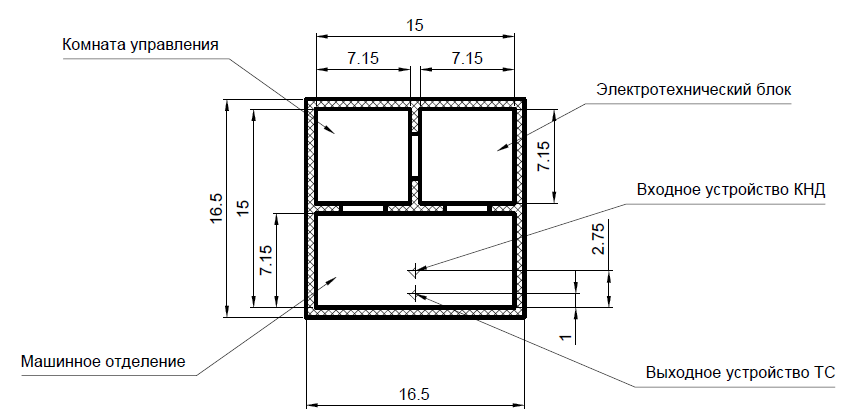
\includegraphics[scale=0.5]{ecology_plan}
	\caption{Схема расчетной области (КНД – компрессор низкого давления, ТС – силовая турбина)}
	\label{img:ecology_plan}
\end{figure}

Соответствующая модель, построенная в программном комплексе АРМ «Акустика» приведен на рис.~\ref{img:ecology_bc}.

\begin{figure}[H]
	\centering
	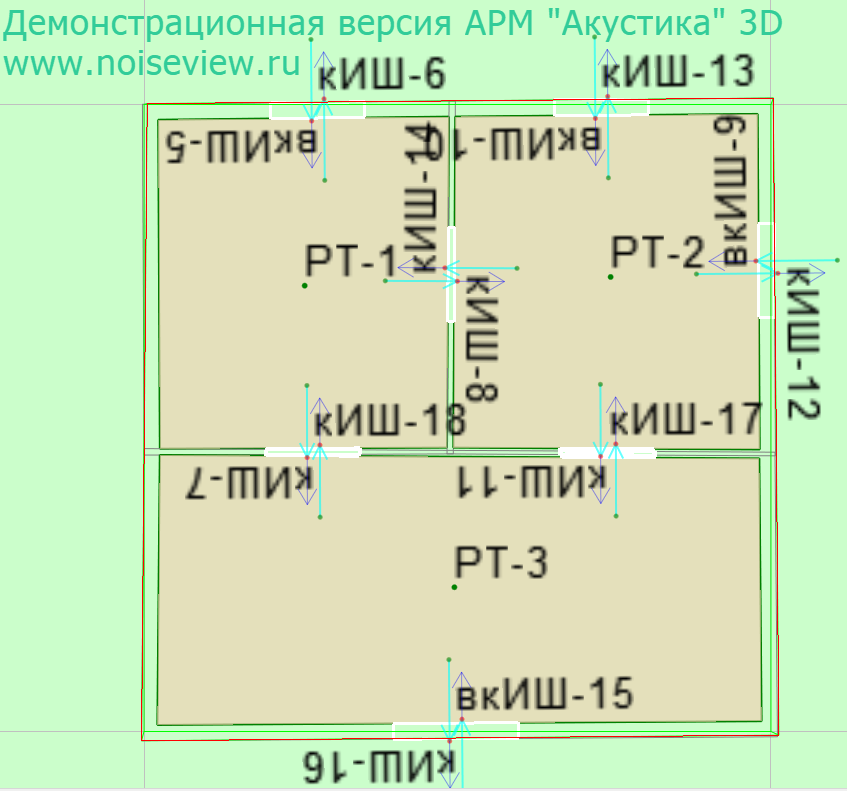
\includegraphics[scale=0.5]{ecology_bc}
	\caption{Расчетная модель, построенная в программном комплексе АРМ "Акустика"}
	\label{img:ecology_bc}
\end{figure}

Для расчета уровней шума использованы шумовые характеристики вентилятора и выходного устройства двигателя НК38-СТ,
идентичные разрабатываемому двигателю. Уровни звукового давления, дБ в октавных полосах со среднегеометрическими частотами, Гц  представлены в таблице 5.2.

\pagebreak
\begin{samepage}
	\begin{longtable}{|c|c|c|c|c|c|c|c|}
		\caption{Уровни звукового давления, дБ в октавных полосах со среднегеометрическим частотами Гц} \label{tab:ecology_noise_power}
		\hline
		\multicolumn{1}{|c}{}& \multicolumn{7}{c|}{Частота, Гц} \\ \hline
		Источник & 31,5 & 63 & 125 & 250 & 500 & 1000 & 2000 \\ \hline
		Вентилятор & 104 & 102 & 103 & 97 & 97 & 94 & 95 \\ \hline
		Выходное устройство & 119 & 117 & 121 & 116 & 114 & 110 & 115 \\ \hline
		\end{longtable}
\end{samepage}

Изолинии звукового давления, полученные в результате расчета показаны на рис.~\ref{img:ecology_result}.

\begin{figure}[H]
	\centering
	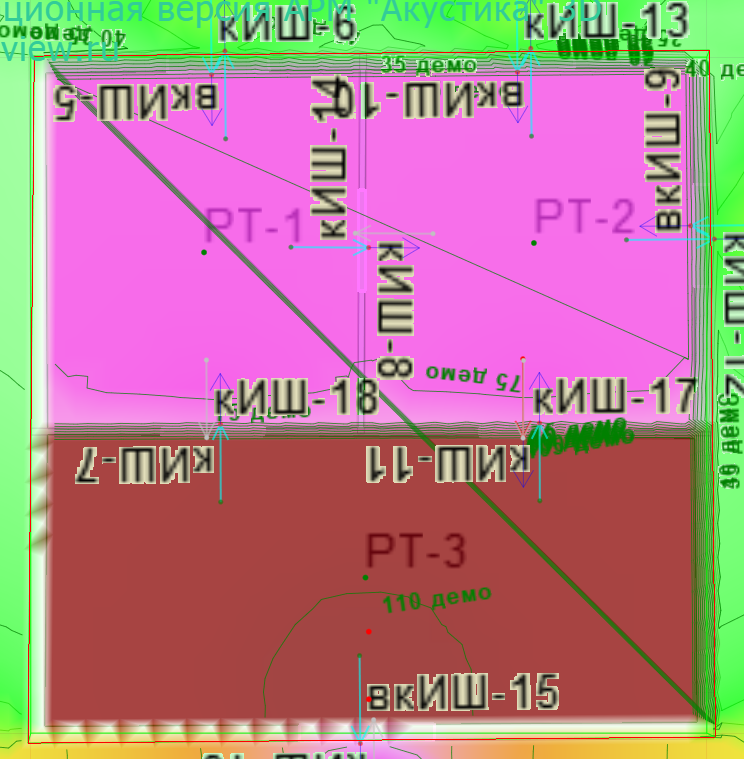
\includegraphics[scale=0.5]{ecology_result}
	\caption{Изолинии звукового давления}
	\label{img:ecology_result}
\end{figure}

Сравнение уровней звукового давления в расчетной точке, находящейся в комнате управления с нормативным (согласно СН 2.2.4/2.1.8.562-
96 таблица 2, строка 4) представлено в таблице 5.3.

\begin{longtable}{|c|c|c|c|c|c|c|c|}
	\caption{Сравнение полученных уровней звукового давления с нормативным} \label{tab:ecology_noise_norm}
	\hline
	\multicolumn{1}{|c}{}& \multicolumn{7}{c|}{Частота, Гц} \\ \hline
	Источник & 31,5 & 63 & 125 & 250 & 500 & 1000 & 2000 \\ \hline
	Норматив & 103 & 91 & 83 & 77 & 73 & 70 & 68 \\ \hline
	Расчетная точка & 83 & 81,5 & 77,3 & 70,1 & 63,8 & 56,4 & 62,5 \\ \hline
\end{longtable}

Из полученных данных следует, что уровень шума на рабочем месте, не превышает нормативного ни в одном из частотных диапазонов.

\subsection{Оценка размера зоны распространения облака горючих газов и паров при аварии} % (fold)
\label{sub:ecology_cloud}

Оценка размера зоны распространения облака горючих газов заключается в определении зоны с концентрацией горючего вещества выше нижнего концентрационного предела воспламенения (НКПВ). Для природного газа эта величина равна 29 мг/л.
Исходные данные для проведения расчета приведены в таблице 5.4.

\pagebreak
\begin{longtable}{|p{6cm}|p{3cm}|p{3cm}|p{4cm}|}
	\caption{Исходные данные для проведения оценки зоны распространения облака горючих газов и паров при аварии} \label{tab:ecology-cloud-input}
	\endfirsthead
	\caption*{\tabcapalign Продолжение таблицы~\thetable}\\[-0.45\onelineskip]
	\hline
	\textbf{Величина} &
	\textbf{Обозначение} &
	\textbf{Размерность} &
	\textbf{Значение} \\ \hline
	\endhead
	\hline
	\textbf{Величина} &
	\textbf{Обозначение} &
	\textbf{Размерность} &
	\textbf{Значение} \\ \hline

	Температура кипения природного газа & $T_к$ & К & 113 \\ \hline
	Теплоемкость природного газа & $C_{pг}$ & $Дж/(кг \cdot К)$ & 3074 \\ \hline
	Теплоемкость воздуха & $C_{pг}$ & $Дж/(кг \cdot К)$ & 1006 \\ \hline
	Газовая постоянная воздуха & $R_в$ & $Дж/(кг \cdot К)$ & 287 \\ \hline
	Газовая постоянная природного газа & $R_в$ & $Дж/(кг \cdot К)$ & 519,6 \\ \hline
	Атмосферное давление & $p_а$ & Па & $1,013 \cdot 10^5$ \\ \hline
	Атмосферная температура & $T_а$ & К & 288 \\ \hline
	Теплота парообразования природного газа & $L_г$ & Дж/кг & $510 \cdot 10^3$ \\ \hline
	Теплота парообразования водяных паров & $L_в$ & Дж/кг & $2256 \cdot 10^3$ \\ \hline
	Температура подстилающей поверхности & $T_{пов}$ & К & 300 \\ \hline
	Относительная влажность & $\psi$ & \% & 50 \\ \hline
	Массовая доля водяных паров & $X$ & - & $9,35 \cdot 10^{-3}$ \\ \hline
	Температура газа в трубопроводе & $T_г$ & К & 275 \\ \hline
	Диаметр трубопровода & $D$ & м & 1,2 \\ \hline
	Длина участка трубопровода между отсечными клапанами & $L$ & м & 6 \\ \hline
	Давление газа в трубопроводе & $p_г$ & Па & $5,6 \cdot 10^6$ \\ \hline
\end{longtable}

Определим массу газа между отсечными клапанами $m_г$, кг:
$$
m_г = \frac{
p_г
}{
R_г T_г
} \cdot \frac{\pi}{4} \cdot D^2 L = \frac{
5,4 \cdot 10^6
}{
519,6 \cdot 275
} \cdot \frac{3,14}{4} \cdot 1,2^2 \cdot 6 = 265,8 кг.
$$
Определим массу воздуха, мгновенно вовлекающуюся в облако углеводородов , кг:
$$
m_в = \frac{
(1 - \delta) \cdot m_г \cdot L_г
}{
C_{pв} \cdot (T_в - T_г) + XL_в
},
$$
где
$$
\delta = 1 - exp\left(
-\frac{
C_{pг}(T_в - T_к)
}{
L_г
}
\right) = 1 - exp\left(
-\frac{
1006 \cdot (288 - 133)
}{
510 \cdot 10^3
}
\right) = 0,65,
$$
таким образом,
$$
m_в = \frac{
(1 - 0,65) \cdot 265,8 \cdot 510 \cdot 10^3
}{
1006 \cdot (288 - 133) + 9,35 \cdot 10^{-3} \cdot 2256 \cdot 10^3 \ кг.
},
$$
Принимается, что образовавшееся облако дрейфует по ветру со скоростью $w_о = 0,6 w$, где $w$ – скорость ветра, и имеет в начальный момент форму цилиндра, высота которого равна его радиусу. С течением времени высота облака уменьшается, а радиус растет.

Скорость ветра зависит от класса устойчивость по Паскуиллу. В данном расчете принимается класс по Паскуиллу B, что соответствует наиболее опасному случаю – наибольшему распространению углеводородного облака. Соответствующая этому классу устойчивости скорость ветра $w = 2 \ м/с$.
Изменение во времени радиуса, высоты облака и концентрации газа в нем в начальной фазе (фаза падения) определяется путем решения систем обыкновенных дифференциальных уравнений:

\[
	\left\{
	\begin{array}{ll}
		\frac{dm_в}{dt} = \rho_в \pi r^2 a_2 a_3 w Ri^{-1} + 2 \rho_в a_1 \frac{dr}{dt} \pi r h \\
		\frac{dT}{dt} = \frac{
		\frac{dm_в}{dt} C_{pв} (T_в - T) + \pi r^2 \cdot (T_{пов} - T)^{1,333}
		}{
		m_в C_{pв} + m_г C_{pг}
		}\\
		\frac{dr}{dt} = a_4 \left(
		\frac{
		dh \cdot (\rho_{г.в.} - \rho_в)
		}{
		\rho_{г.в.}
		}
		\right)^{0,5}
	\end{array}
	\right.
\]
где $m_в$, кг – масса воздуха в облаке, $\rho_в, \ кг/м^3$ – плотность воздуха, $r, \ м$ – радиус облака, $a_1, a_2, a_3, a_4$ – коэффициенты ($a_1=0,7, \ a_2=0,5, \ a_3=1,07, \ a_4=0,3$), $g, \ м/с$ – ускорение свободного падения;

$Ri$ – число Ричардсона, определяемое из соотношения:
$$
Ri = \frac{
\left(
\frac{
5,88h^{0,48}g
}{
a_3^2 w^2
}
\right)^{0,5}
(\rho_{г.в.} - \rho_в)
}{\rho_в};
$$
$h, \ м$ – высота облака, $T, \ к$ – температура облака, $\rho_{г.в.}, \ кг/м^3$ – плотность паровоздушного воздуха.
Для решения системы уравнений необходимо дополнительное соотношение:
$$
\rho_{г.в.} = \frac{
m_в + m_г
}{
\left(
m_в + m_г
\right)
\left(
\frac{T_в}{T}
\right)
}.
$$
В качестве критерия окончания фазы падения принимается выполнение условие
$$
\frac{\rho_{г.в.} - \rho_в}{\rho_{г.в.}} < 10^{-3}.
$$
Зависимость $h=h(t)$ определяется из соотношения:
$$
h(t) = \left(
m_в + m_г
\right)
\left(
\frac{T_в}{T}
\right)
\frac{
1
}{
\pi r(t)^2
}
$$
Концентрация газа в точке с координатами  определяется по формуле:
$$
C(x, y, z) = \frac{
2m_г
}{
(2\pi)^{1,5} \cdot \sigma_y^2 \cdot \sigma_z^2
} \cdot
exp\left(
-\frac{
(x - x_0)^2 + y^2
}{
2\sigma_y^2
}
\right) \cdot
exp\left(
-\frac{
z^2
}{
2\sigma_z^2
}
\right)
$$
где $\sigma_y, \ \sigma_z$ – среднеквадратичные отклонения, зависящие от величины $x_c - x_0$; $x_c, \ м$ – координата центра облака в направлении ветра; $x_0, \ м$ – координата точки окончания фазы падения.

При $x_c = x_0$ принимается $\sigma_{y0}=r/2,14$, $\sigma_{z0}=h/2,14$;

при $x_c \neq x_0$ $\sigma_y^2 = \sigma_{y0}^2 + \sigma_y(x_c - x_0)$, $\sigma_z^2 = \sigma_{z0}^2 + \sigma_z(x_c - x_0)$.

Результатом расчета является пространственное распределение концентраций углеводородного облака. Срез такого
распределения на уровне земли ($z=0$) представлен на рис.~\ref{img:ecology_cloud}.

\begin{figure}[H]
	\centering
	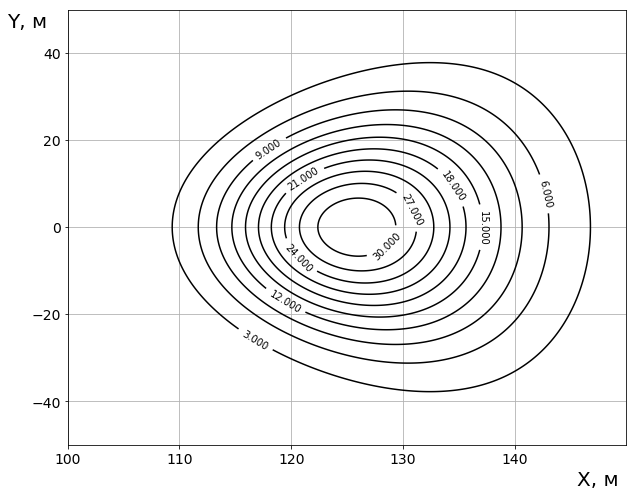
\includegraphics[scale=0.75]{ecology_cloud}
	\caption{Срез распределения концентраций на момент окончания фазы падения}
	\label{img:ecology_cloud}
\end{figure}

Из полученного решения видно, что зона воспламенения по мере движения облака распространяется вплоть до расстояния 130 м по направлению ветра. Следовательно, открытый огонь недопустим в радиусе 130 м от станции.
